%Vyberte nejvhodnější variantu na trhu dostupného řešení a konfrontujte ji s praxí ve vybrané organizaci. 
\section{Výběr nejvhodnější varianty}

Předchozí analýzy prokázaly, že neexistuje řešení, které by dokázalo zastřešit všechny případy užití vlastních zařízení ve firemním prostředí. Proto tato práce bude dále dělit BYOD podle typu zařízení a to na mobilní zařízení jako jsou mobilní telefony či tablety a notebooky.

\section{Výběr řešení pro mobilní telefony a tablety}

\todo{Proc je potreba EMM? Viz specifikace projektu Good}

Trh nástroji v posledních letech výrazně rostl, zároveň se však konsilidoval. \todo{citace https://theictscoop.com/airwatch-consolidates-emm-leadership-in-latest-idc-report-6622602febde   } V grafech \ref{EMM:podil2015} a \ref{EMM:podil2016} je vidět nárůst trhu s EMM mezi lety 2014 a 2015 z 1,4 miliardy dolarů na 1,8 miliardy dolarů, tedy o 26,9 \%. Zároveň je vidět zvyšování tržního podílu velkých hráču. Výrazný vliv měla také akvice společosti Good Technology společností BlackBerry.

 
  \begin{figure}[h]
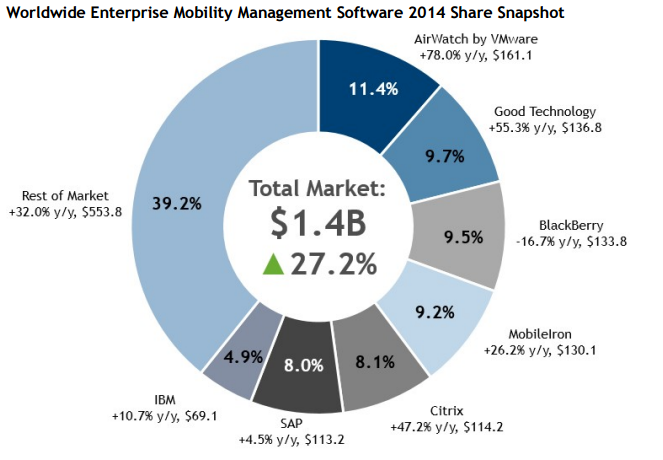
\includegraphics[width=13cm]{img/IDC_EMM}
\caption{Podíl na trhu jednotlivých poskytovatelů EMM v roce 2014 podle IDC Převzato z \cite{}} 
\label{EMM:podil2015}
\centering
\end{figure}\todo{citace http://www.idc.com/getdoc.jsp?containerId=US40430516  }

  \begin{figure}[h]
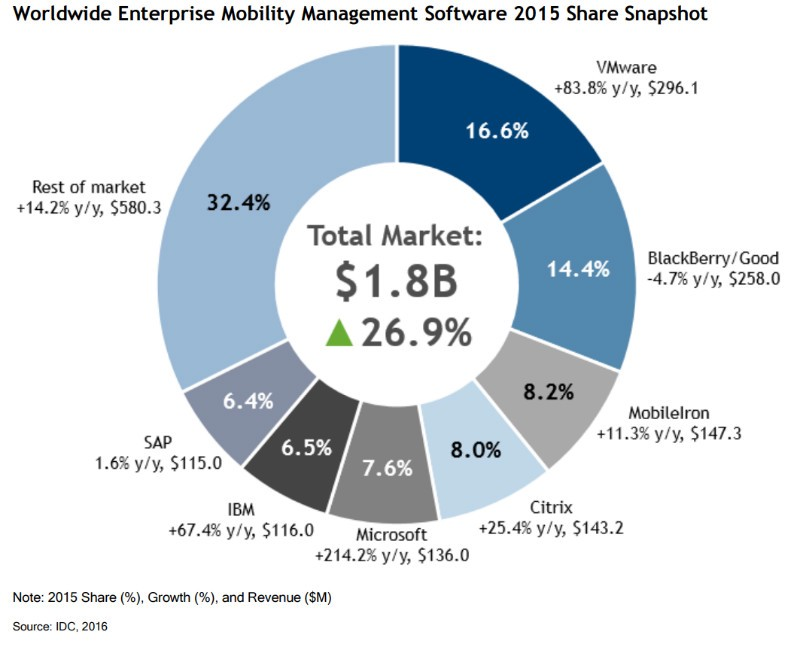
\includegraphics[width=13cm]{img/IDC_EMM_2016}
\caption{Podíl na trhu jednotlivých poskytovatelů EMM v roce 2015 podle IDC Převzato z \cite{}} 
\label{EMM:podil2016}
\centering
\end{figure}\todo{citace https://theictscoop.com/airwatch-consolidates-emm-leadership-in-latest-idc-report-6622602febde   }

Podle magazínu CIOReview bylo v roce 2016 pro BYOD nejslibnějších následujících dvacet poskytovatelů software: Accelion, API Systems, Cyber adAPT, Ericom Software, Excelerate Systems, GSG Telco, High Point Solutions, LANDESK Software,  Mathe, MobileIron, MobilityLab, Movius, RES Software, Sirama Consulting, Skycure, Storgrid, Tangoe, Tyfone, VmWare AirWatch, Zix Corporation.

Některé z nich jsou však příliš úzce zaměřené, či jsou pouze minoritními hráči na trhu. Analýza společnosti Gartner \cite{Gartner_EMM_2016} z roku 2016 pro EMM rozděluje jednotlivé poskytovatele dle jejich postavení na trhu a zároveň zohledňuje jejich schopnost zohlednit v produktu aktuální požadavky trhu a nasměrování produktu k budoucím potřebám zákazníků. Tyto kritéria shrnuje společnost Gartner jako osy "schopnost vykonat" a "úplnost vize" ve svém grafu nazývaném magic quadrant. \ref{EMM:quadrant}



 \begin{figure}[h]
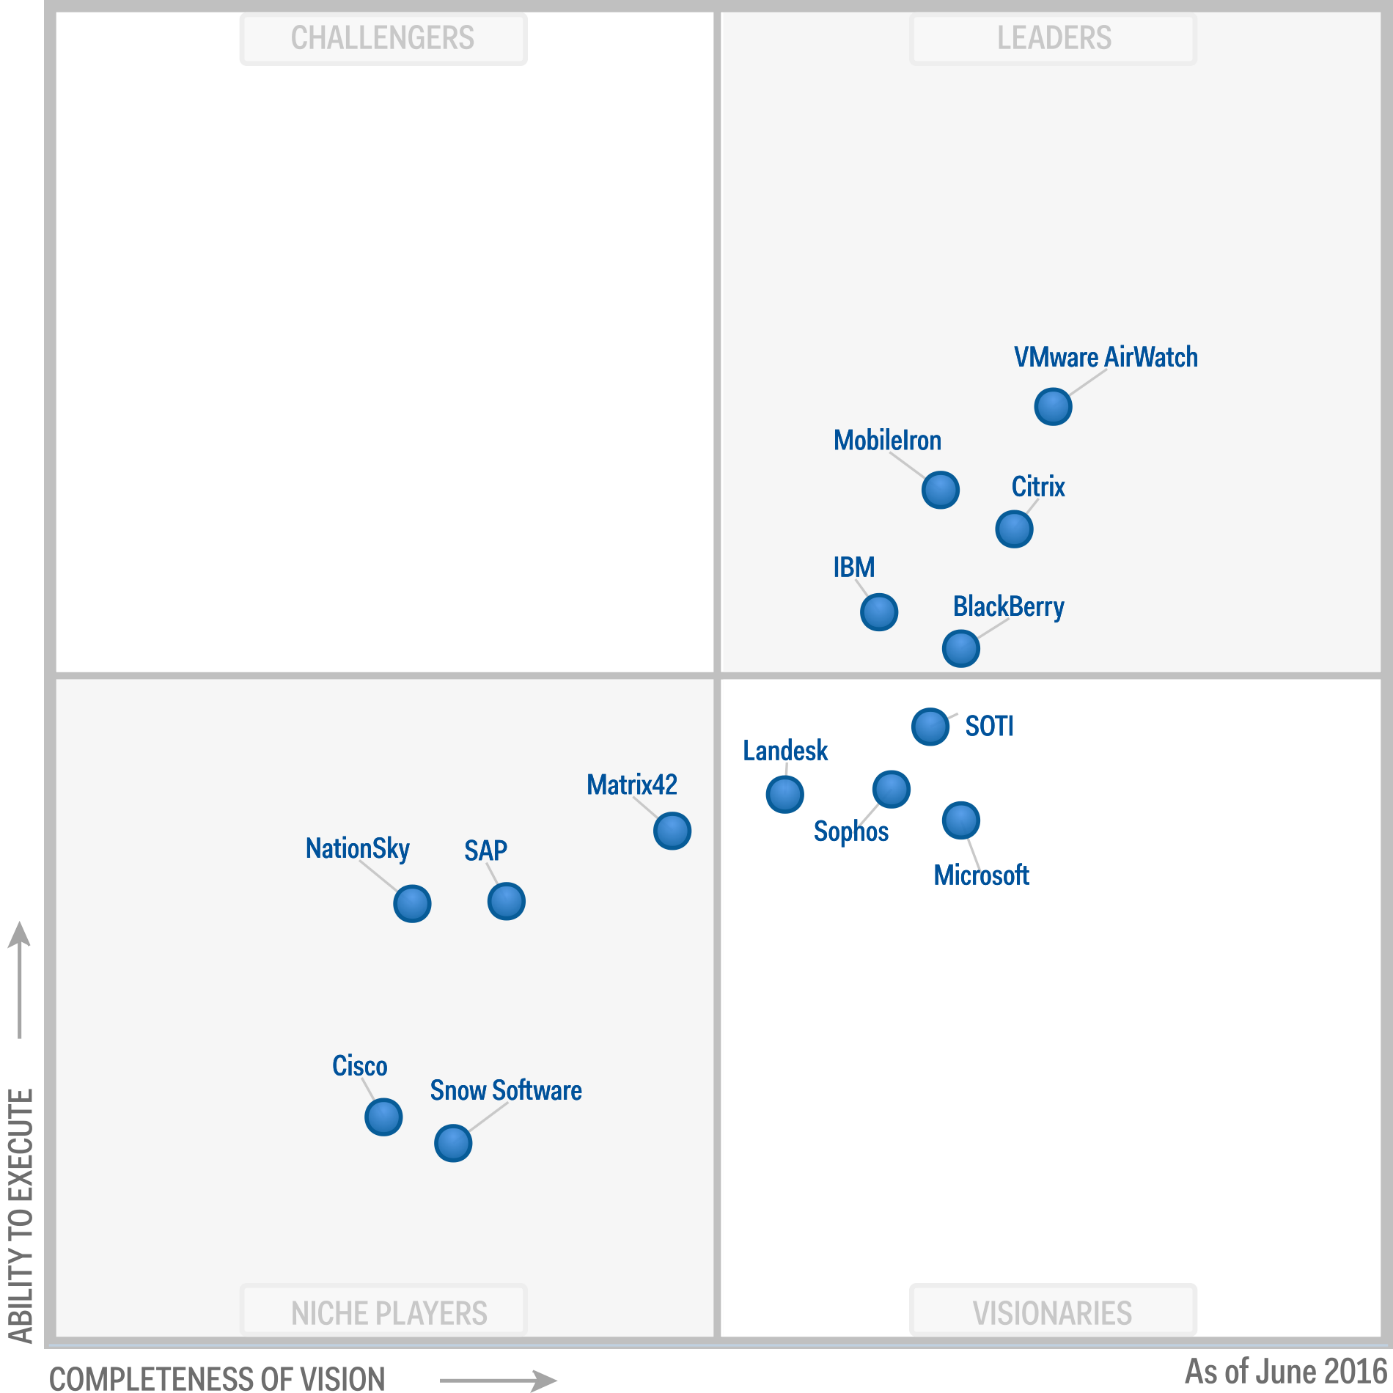
\includegraphics[width=13cm]{img/Gartner_EMM}
\caption{Gartner Magic quadrant. Převzato z \cite{Gartner_EMM_2016}} 
\label{EMM:quadrant}
\centering
\end{figure}\todo{citace}
 %\missingfigure{magic quarter}
 
Následující společnosti se nacházejí v kvadrantu lídrů:


\subsubsection{VMWare Airwatch}
VMWare koupil společnost AirWatch v roce 2014 \todo{citace http://ir.vmware.com/overview/press-releases/press-release-details/2014/VMware-Completes-Acquisition-of-AirWatch/default.aspx}. Od té doby VMWare zařadil tento EMM do svého porfolia a postupně jej integruje s dalšími produkty jakou jsou jeho nástroje pro IAM (Identity and Access Management) a SDN (software-defined networking). AirWatch nabízí širokou podporu pro nástroje třetích stran a je jeden ze zakládajících členů standardu AppConfig. VMWare AirWatch je vhodný pro společnosti, které hledají rozsáhlou funkcionalitu s podporou mnoha platforem.

Podle \todo{citace} byla prokázána nasaditelnost do rozsáhlých prostředí a snadná administrace. Na druhou stranu se objevily problémy s technickou podporou a také nutnost použít řešení od třetí strany pro PIM (Person information management).



\subsubsection{MobileIron}
MobileIron je veřejně obchodovatelná společnost (NASDAQ: MOBL), která jako jedna z posledních soustředí pouze na svůj EMM produkt. Nabízí však širokou podporu aplikací třetích stran a je jedním ze zakládajících členů standardu AppConfig. Společnost je ceněna za schopnost přinášet nové funkce na všechny tři hlavní mobilní platformy a plnění amerických bezpečnostních certifikací. Jedná se o produkt, který nabízí mnoho funkcí, , škálovatelnost, stabilitu a integraci s dalšími aplikacemi.

Řešení nabízí vytváření nástroj pro reporting, pokročilou integraci se SIEM (security information and event management) řešeními třetích stran či správu z mobilního zařízení. Získává kladné ohlasy na svou stabilitu, použitelnost, škálovatelnost a rozsáhlý ekosystém přidružených aplikací AppConnect. MobileIron se drží mezi prvními při nasazování pro nové verze operačních systému.

Na druhou stranu podle \todo{citace} jsou známé případy, kdy zákazníci měli obtíže získat technickou podporu, aplikace Apps@Work nabízejí zastaralý uživatelský zážitek a zároveň existuje nejistota ohledně budoucnosti firmy vzhledem ke změnám ve vrcholém managementu.

\subsubsection{Citrix}
Řešení od společnosti Citrix se skládá z produktů NetScaler, ShareFile a Xen Mobile. Je silné především díky balíku kontejnerizovaných aplikací Worx. ShareFile je kvalitní EFSS (Enterprise file synchronization and sharing) řešení. Obsahuje též uživatelsky přívětivé DLP (Data loss prevention).XenMobile je vhodný pro společnosti s existující infrastrukturou od Citrixu nebo pro ty co požadují široké spektrum funkcí.

Společnost Gartner zaznamenala probléby u nasazení XenMobile jako SaaS (Software as a service) u velkých projektů (tj. více než 20000 zařízení). Přestože XenMobile nabízí možnost virtualizace Windows aplikací pro mobilní zařízení, použitelnost je na na mobilních zařízeních sporná, vzhledem k dotykové povaze ovládání uživatelského rozhraní. 


\subsubsection{IBM}
IBM nabízí komletní malík EMM nástrojů MaaS360. Podporuje všechny významné operační systémy, nabízí dobrou spolupráci s dalším bezpečnostním software od IBM. Jedná se o produkt, který má velký záběr co se týče funkcionality, ale přitom je snadno nasaditelný.



\subsubsection{BlackBerry}
BlackBerry nyní prodává svůj nástroj jako Good Secure EMM Suite. Skládá se z BES12, Good collaboration apps, Good dynamics a WatchDox Enterprise. Produkty pod značkou Good a WatchDox získala Blacberry akvizicemi které byly dokončeny v roce 2015. \todo{citace http://global.blackberry.com/en/company/newsroom/press?id=1998017} \todo{http://global.blackberry.com/en/company/newsroom/press?id=1946553}

Podle agentury Gartner je Good Secure EMM Suite vhodný pro organizace s přísnými požadavky na bezpečnost či působící v regulovaném sektoru. Těm nabízí silnou sadu nástrojů pro ochranu. Zároveň existuje silná podpora pro starší verze software od BlackBerry. Nástroj Good Work nabízí jeden z nejlepších zabezbečených Personal information manager (PIM) nástrojů. Podpora od BlackBerry získává mnoho kladných hodnocení od zákazníků. 

Vícevrstvá cloudová verze produktu BES12 umisťuje data do datacenter ve dvou lokacích a to Kanady a Nizozemí. To by mohl být pro některé bezpečnostní politiky problém. Zároveň u balíku od společnosti BlackBerry dochází k roztříštěnosti služeb mezi jednotlivými produkty.

\todo{funkce a tak}

Další řešení:

\subsubsection{Cisco}
Cisco se dostalo mezi společnosti nabízející MDM software akvizicí společnosti Meraki v roce 2012 \todo{citace https://newsroom.cisco.com/press-release-content?articleId=1118649}. Kromě řešení pro Android a iOS nabízí také podporu pro Windows a MAC OS X. Nabízí hlubokou integraci do síťové ingrastruktury. Správa produktu nabízí velice jednoduché a přívětivé uživatelské rozhraní. Cenově se jedná o levnější řešení než většina konkurence.

Výhody integrace do síťové infrastruktury je možné využít pouze v případě, že organizace používá sítovou infrastrukturu od Cisco/Meraki. Meraki neobsahuje všechny součásti EMM, soutředí se pouze na MDM.



\subsubsection{Microsoft}
EMM produkt od Microsoftu se nazývá Enterprise Mobility Suite. Skládá se z Microsoft Intune, Azure Active Directory Premium, Advanced Threat Analytics a Azure Rights Management. MDM a MAM služby jsou soustředěny v Microsoft Intune. Toto řešení je nabízeno pouze služba v cloudu. Řešení od Microsoftu je vhodné pro společnosti, které nemají vysoké nároky na správu a používají Office 365 nebo Azure Active Directory.

\subsubsection{Landesk}
Landesk se zaměřuje především na UEM (User Evironment Management) a jeho řešení Landesk Mobility Suite tak zapadá do jeho portfolia jako doplněk pro mobilní zařízení. Je tedy vhodné především pro firmy, které mají potřebu spravovat desktopové prostředí a mobilní zařízení zároveň.

\subsubsection{Další řešení}
Ostatní řešení byla v \todo{citace} byla prezentována jako mající příliš úzké zaměření, nedostatečnou funkcionalitu nebo nevhodnost pro nasazení ve větším měřítku


\section{Výběr řešení pro notebooky}

Vzhledem k požadavkům na bezpečnost a dodržování přísných firemních politik v bance a zároveň k potřebě přístupů k různým typům software a aplikací se zdá jako jediné vhodné řešení BYOD virtualizace desktopu. Způsobů, jakými může virtualizace sloužit pro řešení BYOD je více.

Analýza \ref{Forreste_Wave} z září roku 2015 od společnosti Forrester se zaměřuje na virtuální desktopy umístěné na vlastním serveru. Výhodou oproti DaaS řešení je, že aplikace i data jsou pod úplnou kontrolou IT oddělení, což snižuje riziko ztráty nebo krádeže dat. Nevýhodou těchto řešení může být problémová funkčnost některých periferních zařízení, jako jsou webové kamery nebo tiskárny. Dále jsou tato řešení velmi náročná na stabilitu a rychlost internetového připojení a to především u graficky náročnějších aplikací. 

 \begin{figure}[h]\label{Forrester_Wave}
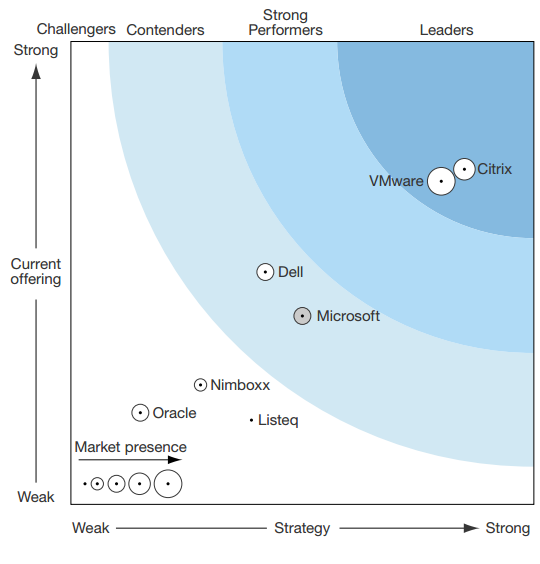
\includegraphics[width=13cm]{img/Forrester_Wave}
\caption{The Forrester Wave: Virtuání desktopy umístěné na serveru} 
\label{EMM:quadrant}
\centering
\end{figure}\todo{citace https://www.citrix.com/content/dam/citrix/en\_us/documents/products-solutions/forrester-wave-server-hosted-virtual-desktops-q3-2015.pdf}

Průzkum trhu od společnosti IDC z roku 2016 \todo{citovat IDC_VM} \ref{IDC_VM} má širší zaměření, a to na poskytovatele VCC (Virtual Client Computing). Ty definuje jako poskytovatele kteří tvoří a prodávají software pro virtualizaci se zaměřením na centralizované virtuální desktopy, distribuované virtuální desktopy a software pro virtuální uživatelské sezení (VUS).

 \begin{figure}[h]\label{IDC_VM}
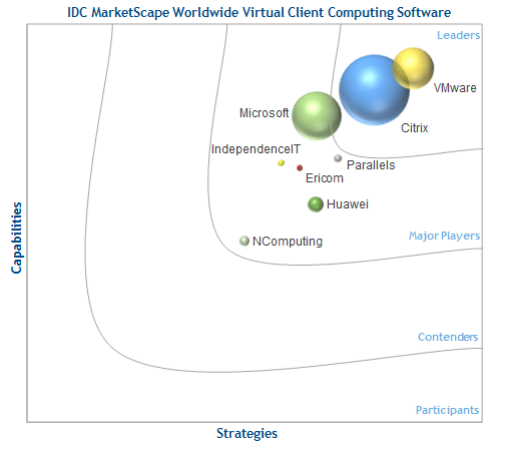
\includegraphics[width=13cm]{img/IDC_VM}
\caption{IDC MarketScape: Hodnocení dodavatelů klientů pro virtualizovaný software } 
\label{EMM:quadrant}
\centering
\end{figure}\todo{citace http://campaign.vmware.com/imgs/GlobalCampaigns/39249/IDC_MarketScape_Worldwide_Virtual_Client_Computing_Software_2016_Vendor_Assessment.pdf}

\subsection{Citrix}
Řešení XenDesktop se vyznačuje podporou vlastního protokolu HDX \todo{citace https://www.citrix.com/blogs/2014/08/18/citrix-xendesktopxenapp-what-is-hdx-its-not-just-ica/} díky kterému se snaží o adaptivní kompresi, de-duplikaci síťového provozu a přesměrování tíhy renderování dle okolností na klienta a to na všech podporovaných platformách. Dále podporuje vícenásobné 4k monitory a pokročilé funkce pro multimedia a videokonference. Výhodou je podpora amerického bezpečnostního standardu FIPS 140-2.
Podle \todo{citace forrestera} má XenDesktop výborné uživatelské hodnocení, avšak technická podpora je pomalá.


\subsection{VMWare}
VMWare nabízí produkt VMWare Horizon View. Použitý protokol je PCoIP od firmy Teradici. Je vhodný v kombinaci serverem vSphere, kdy nabízí dobrou integraci. Nabízí též škálování do cloudu v kooperaci s řešením Horizon Air. Taktéž moduly software od VMWare splňují bezpečnostní standard FIPS 140-2. \todo{citace http://www.vmware.com/security/certifications/fips.html}. Horizon View je také možné zakoupit jako součást kompletního balíku, který obsahuje taktéž Horizon Flex pro offline použití. Podle \todo{zase ocitovat forrestera} hodnotí zákazníci produkt jako dobrý s několika problémy, jako například nutnost použití příkazové řádky pro některá nastavení.


\subsection{Microsoft}

\subsection{Oracle}
Oracle nabízí nástroj Secure Global Desktop, který je možné použít s různými hypervizory, je ovšem optimalizovaný pro Oracle. Hlavní devízou řešení je kvalitní konzole pro správu Oracle Enterprise Manager. Podle \todo{zase cituj forestra} toto řešení není vhodné pro případy užití mimo prostředí s vysokým podílem aplikací od Oracle.



%Konzultujte navrhované řešení se zástupci vybrané organizace a stanovte doporučení pro nasazení. 
\section{Hodnocení navrhované varianty zástupci KB}

%Navrhněte nasazení řešení BYOD. 
\section{Návrh řešení}


%Zhodnoťte uskutečnitelnost řešení a analyzujte benefity a rizika spojená se zavedením navrženého konceptu.
\section{Analýza navrženého řešení}